\section{Wymagania funkcjonalne}

\subsection{Obsługa logistyczna}
\subsubsection*{Opis}
Moduł zawiera funkcjonalności z zakresu obsługi transportu przesyłek.

\subsubsection*{Przypadki użycia}
\begin{figure}[H]
\centering
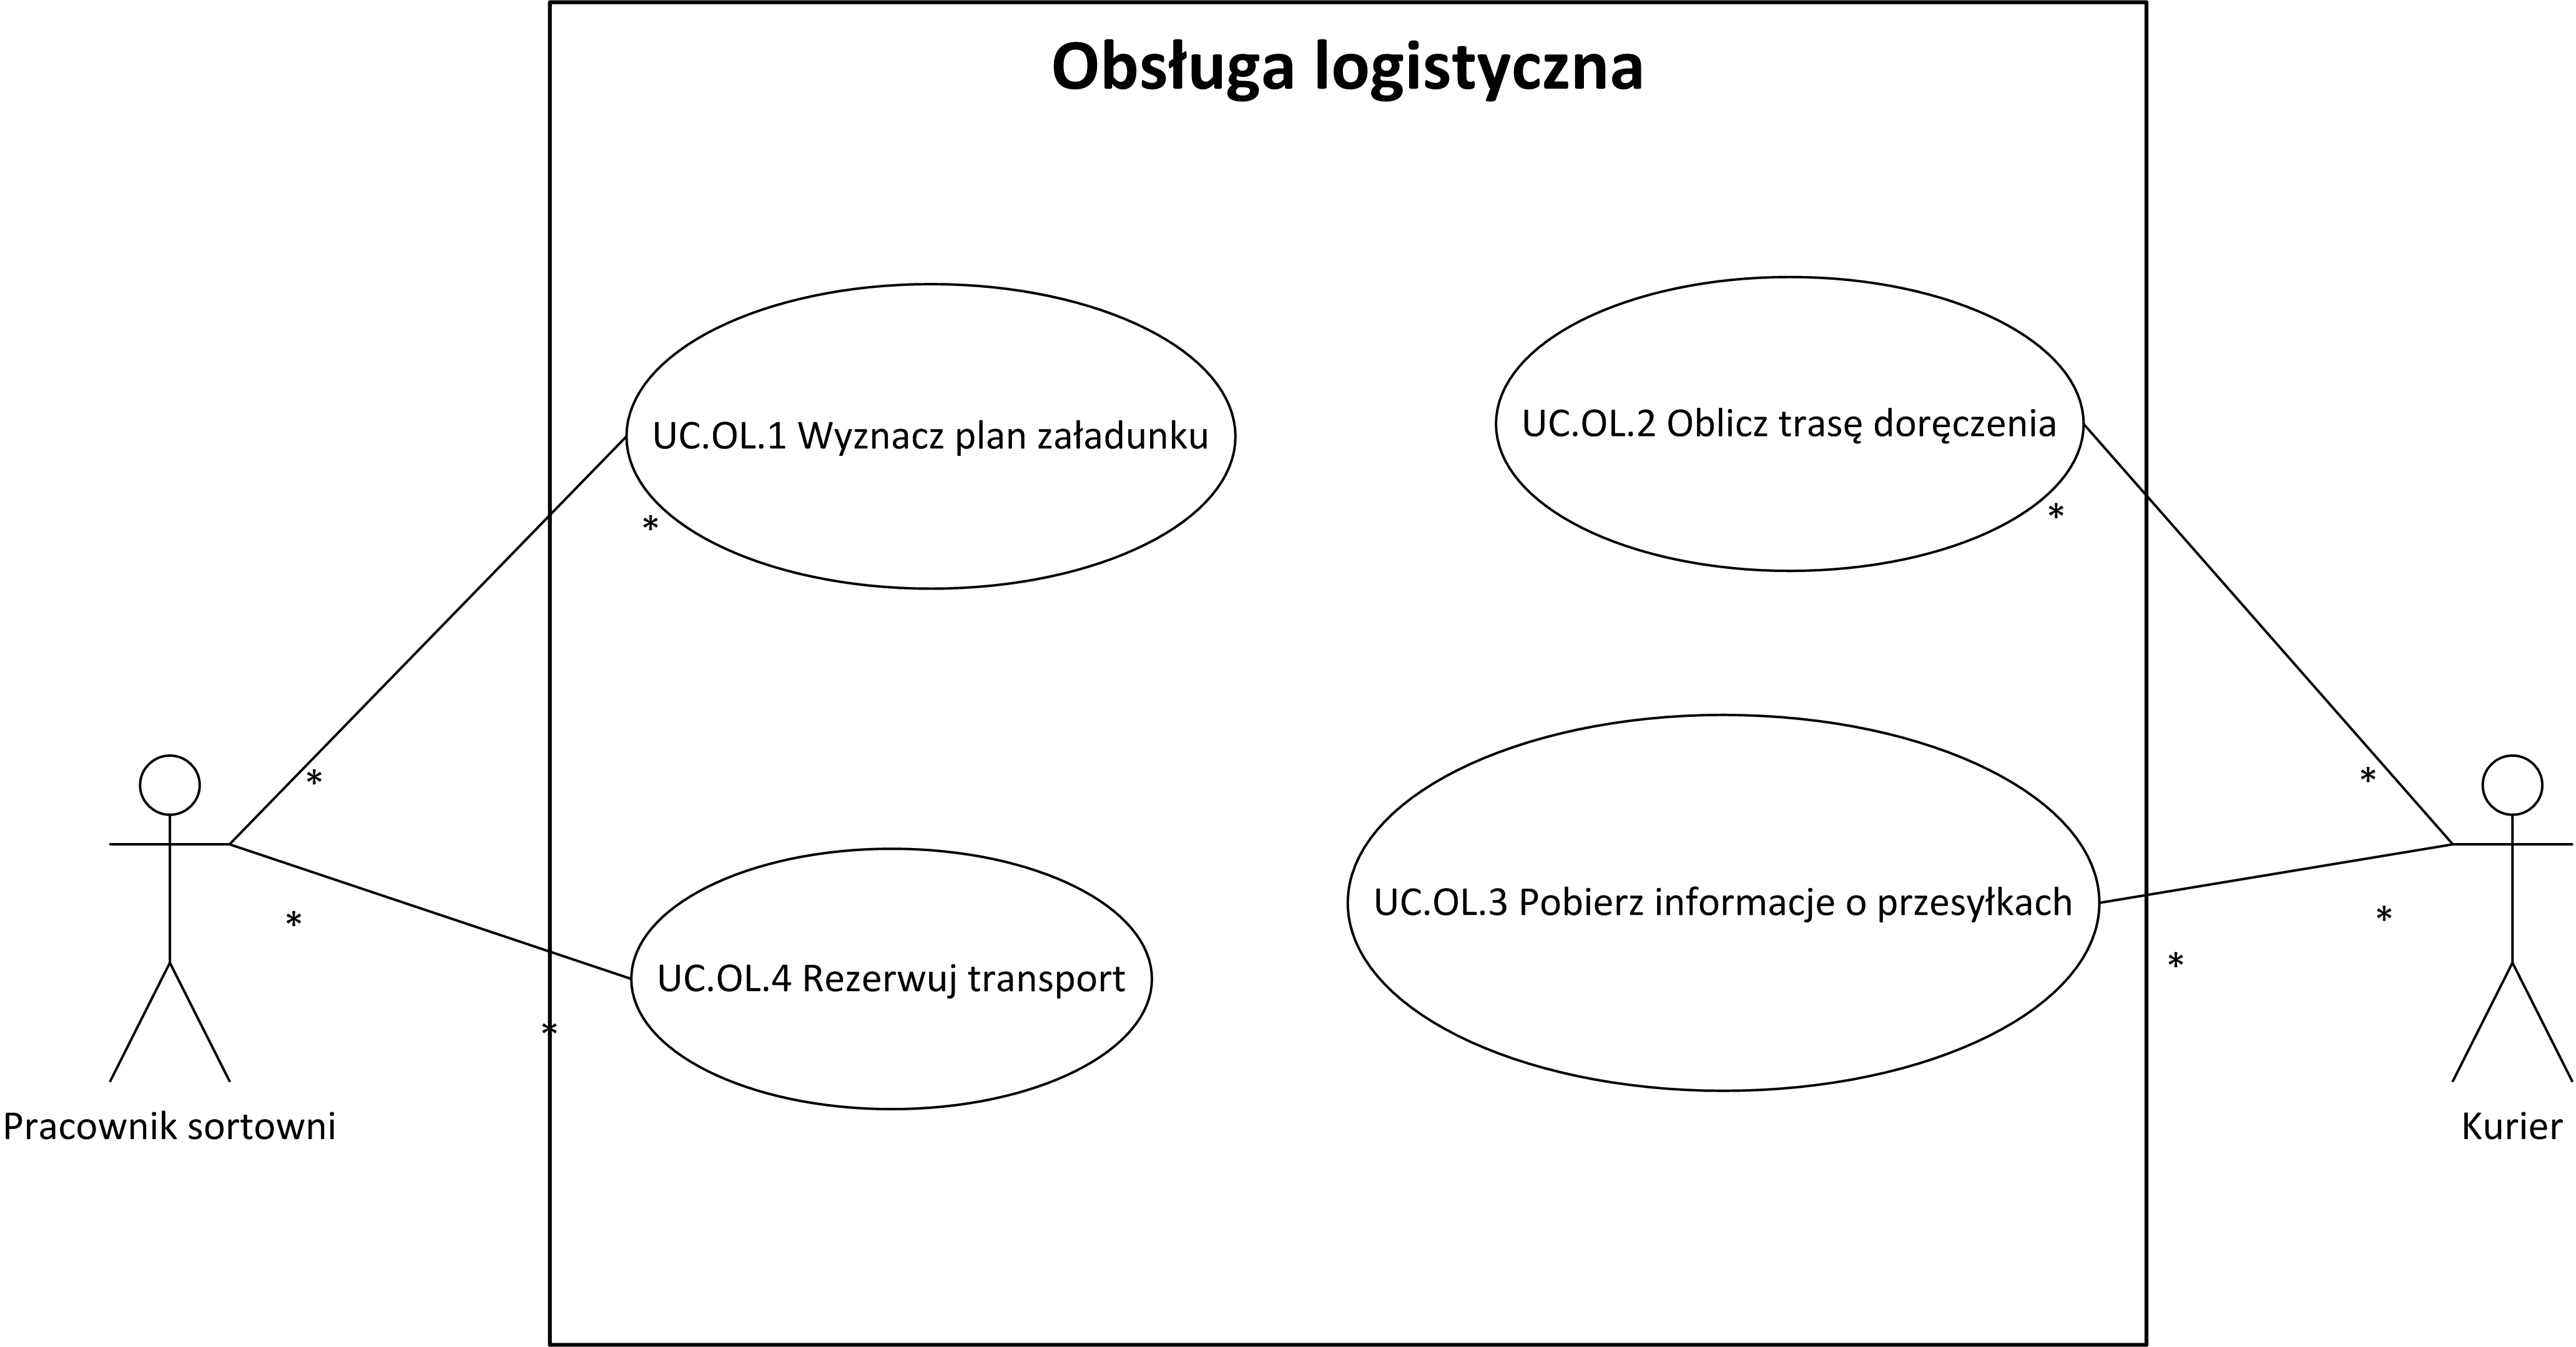
\includegraphics[width=\textwidth]{img/obs_log_uc}
\end{figure}

\subsubsection*{Scenariusze przypadków użycia}
\begin{center}
\begin{longtable}[h]{|p{1.6cm}|p{13.5cm}|}
\hline
\textbf{ID:} & UC.OL.1 \\ \hline
\textbf{Nazwa:} & Wyznacz plan załadunku \\ \hline
\multicolumn{2}{|p{15.1cm}|}{\textbf{Aktorzy główni:} Pracownik sortowni} \\
\multicolumn{2}{|p{15.1cm}|}{\textbf{Aktorzy pomocniczy:} \textit{brak}} \\
\multicolumn{2}{|p{15.1cm}|}{\textbf{Poziom:} Użytkownika} \\
\multicolumn{2}{|p{15.1cm}|}{\textbf{Priorytet:} Wysoki} \\
\hline
\multicolumn{2}{|p{15.1cm}|}{\textbf{Opis:}} \\
\multicolumn{2}{|p{15.1cm}|}{
Pracownik sortowni chce uzyskać plan załadunku przesyłek, które oczekują na doręczenie.
} \\ \hline
\multicolumn{2}{|p{15.1cm}|}{\textbf{Wyzwalacze:}} \\
\multicolumn{2}{|p{15.1cm}|}{
Wybranie odpowiedniej opcji w aplikacji klienckiej.
} \\ \hline
\multicolumn{2}{|p{15.1cm}|}{\textbf{Warunki początkowe:}} \\
\multicolumn{2}{|p{15.1cm}|}{
Aktor musi być zalogowany do SWPFK.
} \\ \hline
\multicolumn{2}{|p{15.1cm}|}{\textbf{Warunki końcowe:}} \\
\multicolumn{2}{|p{15.1cm}|}{
System wyświetla przygotowany plan załadunku przesyłek.
} \\ \hline
\multicolumn{2}{|p{15.1cm}|}{\textbf{Scenariusz główny:}} \\
\multicolumn{2}{|p{15.1cm}|}{
\begin{enumerate}
\item Aktor wybiera opcję ''Oblicz plan załadunku''.
\item System wyświetla listę przesyłek, które oczekują na doręczenie. Domyślnie wszystkie przesyłki są zaznaczone.
\item Aktor odznacza przesyłki, które chce wyłączyć z doręczenia.
\item Aktor wyzwala przeliczanie wybierając funkcję ''Wyznacz plan''.
\item System gromadzi parametry wybranych przesyłek.
\item System pobiera informacje o pojazdach dostępnych do doręczenia.
\item System wyznacza plan załadunku uwzględniając pobrane informacje oraz możliwe trasy doręczeń.
\item System prezentuje plan w tabelach reprezentujących pojazdy, które zawierają wyszczególnione przesyłki w kolejności jakiej powinny być załadowane do pojazdu.
\end{enumerate}
} \\ \hline
\multicolumn{2}{|p{15.1cm}|}{\textbf{Scenariusze alternatywne i rozszerzenia:}} \\
\multicolumn{2}{|p{15.1cm}|}{
3.a Aktor odznaczył wszystkie możliwe przesyłki. \newline
3.a.1 System prezentuje ostrzeżenie, że nie wybrano żadnej przesyłki. \newline
3.a.2 Aktor zaznacza wybrane przesyłki. \newline
3.a.3 Powrót do punktu 4 scenariusza głównego. \newline
\newline
7.a Wyznaczenie planu załadunku nie powiodło. \newline
7.a.1 System prezentuje informacje o błędzie podczas wyznaczania planu. \newline
7.a.2 Aktor koryguje listę przesyłek do doręczenia. \newline
7.a.3 Powrót do punktu 4 scenariusza głównego.
} \\ \hline
\multicolumn{2}{|p{15.1cm}|}{\textbf{Wyjątki:}} \\
\multicolumn{2}{|p{15.1cm}|}{
System posiada nieaktualne informacje o pojazdach, co powoduje wyznaczenie błędnego planu.
} \\ \hline
\multicolumn{2}{|p{15.1cm}|}{\textbf{Dodatkowe wymagania:}} \\
\multicolumn{2}{|p{15.1cm}|}{
\textit{brak}
} \\
\hline
\end{longtable}
\end{center}

\begin{center}
\begin{longtable}[h]{|p{1.6cm}|p{13.5cm}|}
\hline
\textbf{ID:} & UC.OL.2 \\ \hline
\textbf{Nazwa:} & Oblicz trasę doręczenia \\ \hline
\multicolumn{2}{|p{15.1cm}|}{\textbf{Aktorzy główni:} Kurier} \\
\multicolumn{2}{|p{15.1cm}|}{\textbf{Aktorzy pomocniczy:} \textit{brak}} \\
\multicolumn{2}{|p{15.1cm}|}{\textbf{Poziom:} Użytkownika} \\
\multicolumn{2}{|p{15.1cm}|}{\textbf{Priorytet:} Wysoki} \\
\hline
\multicolumn{2}{|p{15.1cm}|}{\textbf{Opis:}} \\
\multicolumn{2}{|p{15.1cm}|}{
Kurier chce wygenerować trasę doręczenia przesyłek.
} \\ \hline
\multicolumn{2}{|p{15.1cm}|}{\textbf{Wyzwalacze:}} \\
\multicolumn{2}{|p{15.1cm}|}{
Aktor wybiera opcję ''Wyznacz trasę doręczenia'' w aplikacji mobilnej.
} \\ \hline
\multicolumn{2}{|p{15.1cm}|}{\textbf{Warunki początkowe:}} \\
\multicolumn{2}{|p{15.1cm}|}{
1. Został wygenerowany plan załadunku pojazdów. \newline
2. Kurier wprowadził numer pojazdu do aplikacji mobilnej.
} \\ \hline
\multicolumn{2}{|p{15.1cm}|}{\textbf{Warunki końcowe:}} \\
\multicolumn{2}{|p{15.1cm}|}{
System prezentuje obliczoną trasę doręczenia.
} \\ \hline
\multicolumn{2}{|p{15.1cm}|}{\textbf{Scenariusz główny:}} \\
\multicolumn{2}{|p{15.1cm}|}{
\begin{enumerate}
\item Aktor wybiera opcję ''Wyznacz trasę doręczenia''.
\item Aplikacja mobilna przesyła żądanie do modułu serwerowego o obliczenie trasy doręczenia.
\item Moduł serwerowy wyznacza trasę na podstawie informacji o przesyłkach znajdujących się w pojeździe.
\item Moduł serwerowy przesyła wyznaczoną trasę do aplikacji klienckiej.
\item Aplikacja mobilna prezentuje trasę doręczenia.
\item Aktor wybiera opcję ''Zapisz trasę''.
\item Aplikacja mobilna zapisuje wyznaczoną trasę.
\end{enumerate}
} \\ \hline
\multicolumn{2}{|p{15.1cm}|}{\textbf{Scenariusze alternatywne i rozszerzenia:}} \\
\multicolumn{2}{|p{15.1cm}|}{
3.a Wystąpił błąd podczas obliczania trasy. \newline
3.a.1 Moduł serwerowy przesyła informacje o zaistniałym błędzie. \newline
3.a.2 Aplikacja mobilna prezentuje informacje o błędzie. \newline
3.a.3 Przypadek użycia kończy się.
} \\ \hline
\multicolumn{2}{|p{15.1cm}|}{\textbf{Wyjątki:}} \\
\multicolumn{2}{|p{15.1cm}|}{
Terminal mobilny nie ma połączenia z modułem serwerowym.
} \\ \hline
\multicolumn{2}{|p{15.1cm}|}{\textbf{Dodatkowe wymagania:}} \\
\multicolumn{2}{|p{15.1cm}|}{
\textit{brak}
} \\
\hline
\end{longtable}
\end{center}

\begin{center}
\begin{longtable}[h]{|p{1.6cm}|p{13.5cm}|}
\hline
\textbf{ID:} & UC.OL.3 \\ \hline
\textbf{Nazwa:} & Pobierz informacje o przesyłkach \\ \hline
\multicolumn{2}{|p{15.1cm}|}{\textbf{Aktorzy główni:} Kurier} \\
\multicolumn{2}{|p{15.1cm}|}{\textbf{Aktorzy pomocniczy:} \textit{brak}} \\
\multicolumn{2}{|p{15.1cm}|}{\textbf{Poziom:} Użytkownika} \\
\multicolumn{2}{|p{15.1cm}|}{\textbf{Priorytet:} Średni} \\
\hline
\multicolumn{2}{|p{15.1cm}|}{\textbf{Opis:}} \\
\multicolumn{2}{|p{15.1cm}|}{
Kurier chce pobrać na terminal mobilny informacje o przesyłkach, które ma doręczyć.
} \\ \hline
\multicolumn{2}{|p{15.1cm}|}{\textbf{Wyzwalacze:}} \\
\multicolumn{2}{|p{15.1cm}|}{
Aktor wybiera opcję ''Pobierz informacje o przesyłkach''.
} \\ \hline
\multicolumn{2}{|p{15.1cm}|}{\textbf{Warunki początkowe:}} \\
\multicolumn{2}{|p{15.1cm}|}{
Został wygenerowany plan załadunku pojazdów.
} \\ \hline
\multicolumn{2}{|p{15.1cm}|}{\textbf{Warunki końcowe:}} \\
\multicolumn{2}{|p{15.1cm}|}{
Informacje o przesyłkach zostają zapisane na terminalu mobilnym.
} \\ \hline
\multicolumn{2}{|p{15.1cm}|}{\textbf{Scenariusz główny:}} \\
\multicolumn{2}{|p{15.1cm}|}{
\begin{enumerate}
\item Aktor wybiera opcję ''Pobierz informacje o przesyłkach''.
\item Aplikacja mobilna przesyła żądanie do modułu serwerowego.
\item Moduł serwerowy pobiera informacje o przesyłkach i przesyła je do aplikacji mobilnej.
\item Aplikacja mobilna zapisuje otrzymane informacje.
\item Aplikacja mobilna prezentuje otrzymane dane.
\end{enumerate}
} \\ \hline
\multicolumn{2}{|p{15.1cm}|}{\textbf{Scenariusze alternatywne i rozszerzenia:}} \\
\multicolumn{2}{|p{15.1cm}|}{
\textit{brak}
} \\ \hline
\multicolumn{2}{|p{15.1cm}|}{\textbf{Wyjątki:}} \\
\multicolumn{2}{|p{15.1cm}|}{
Terminal mobilny nie ma połączenia z modułem serwerowym.
} \\ \hline
\multicolumn{2}{|p{15.1cm}|}{\textbf{Dodatkowe wymagania:}} \\
\multicolumn{2}{|p{15.1cm}|}{
\textit{brak}
} \\
\hline
\end{longtable}
\end{center}

\begin{center}
\begin{longtable}[h]{|p{1.6cm}|p{13.5cm}|}
\hline
\textbf{ID:} & UC.OL.4 \\ \hline
\textbf{Nazwa:} & Rezerwuj transport \\ \hline
\multicolumn{2}{|p{15.1cm}|}{\textbf{Aktorzy główni:} Pracownik sortowni} \\
\multicolumn{2}{|p{15.1cm}|}{\textbf{Aktorzy pomocniczy:} 
Zewnętrzna firma transportowa} \\
\multicolumn{2}{|p{15.1cm}|}{\textbf{Poziom:} Użytkownika} \\
\multicolumn{2}{|p{15.1cm}|}{\textbf{Priorytet:} Wysoki} \\
\hline
\multicolumn{2}{|p{15.1cm}|}{\textbf{Opis:}} \\
\multicolumn{2}{|p{15.1cm}|}{
Pracownik sortowni chce zarezerwować transport w celu przewiezienia oczekujących przesyłek.
} \\ \hline
\multicolumn{2}{|p{15.1cm}|}{\textbf{Wyzwalacze:}} \\
\multicolumn{2}{|p{15.1cm}|}{
Aktor wybiera opcję ''Rezerwuj transport'' w aplikacji klienckiej.
} \\ \hline
\multicolumn{2}{|p{15.1cm}|}{\textbf{Warunki początkowe:}} \\
\multicolumn{2}{|p{15.1cm}|}{
\textit{brak}
} \\ \hline
\multicolumn{2}{|p{15.1cm}|}{\textbf{Warunki końcowe:}} \\
\multicolumn{2}{|p{15.1cm}|}{
Transport dla wyznaczonych przesyłek zostaje zarezerwowany we flocie Firmy Kurierskiej lub flocie firmy zewnętrznej.
} \\ \hline
\multicolumn{2}{|p{15.1cm}|}{\textbf{Scenariusz główny:}} \\
\multicolumn{2}{|p{15.1cm}|}{
\begin{enumerate}
\item Aktor wybiera opcję ''Rezerwuj transport'' w aplikacji klienckiej.
\item Aplikacja kliencka prezentuje listę przesyłek oczekujących na przesłanie do innych sortowni. Domyślnie wszystkie przesyłki są zaznaczone.
\item Aktor odznacza przesyłki, które nie mają zostać przesłane.
\item Aplikacja kliencka przesyła żądanie rezerwacji do modułu serwerowego.
\item Moduł serwerowy wyznacza sieć połączeń na jakich trzeba przetransportować wybrane przesyłki.
\item Moduł serwerowy pobiera informacje o dostępnej flocie wewnętrznej.
\item Moduł serwerowy komunikuje się z systemami zewnętrznych firm transportowych w celu pobrania informacji o dostępnej flocie.
\item Moduł serwerowy wyznacza listę pojazdów jakie należy zarezerwować i przesyła ją do aplikacji klienckiej.
\item Aplikacja kliencka prezentuje wyznaczony plan przewozu.
\item Aktor zatwierdza wyznaczony plan.
\item Moduł serwerowy rezerwuje pojazdy we flocie wewnętrznej oraz przesyła żądania rezerwacji do zewnętrznych firm.
\item Moduł serwerowy generuje potwierdzenie pomyślnej rezerwacji pojazdów oraz przesyła je do aplikacji klienckiej.
\item Aplikacja kliencka prezentuje potwierdzenie rezerwacji.
\end{enumerate}
} \\ \hline
\multicolumn{2}{|p{15.1cm}|}{\textbf{Scenariusze alternatywne i rozszerzenia:}} \\
\multicolumn{2}{|p{15.1cm}|}{
8.a Wyznaczenie listy pojazdów jest niemożliwe z powodu braku ich dostępności. \newline
8.a.1 Moduł serwerowy generuje ostrzeżenie i przesyła je do aplikacji klienckiej. \newline
8.a.2 Aplikacja kliencka prezentuje informacje o niepowodzeniu. \newline
8.a.3 Przypadek użycia kończy się.\newline
\newline
11.a Rezerwacja pojazdów została odrzucona. \newline
11.a.1 Moduł serwerowy przesyła powód odrzucenia do aplikacji klienckiej.\newline
11.a.2 Aplikacja kliencka prezentuje informacje o niepowodzeniu. \newline
11.a.3 Aktor wybiera opcję ''Spróbuj ponownie''. \newline
11.a.4 Powrót do punktu 4 scenariusza głównego.
} \\ \hline
\multicolumn{2}{|p{15.1cm}|}{\textbf{Wyjątki:}} \\
\multicolumn{2}{|p{15.1cm}|}{
Aplikacja kliencka nie ma połączenia z modułem serwerowym.
} \\ \hline
\multicolumn{2}{|p{15.1cm}|}{\textbf{Dodatkowe wymagania:}} \\
\multicolumn{2}{|p{15.1cm}|}{
\textit{brak}
} \\
\hline
\end{longtable}
\end{center}

\subsection{Obsługa finansowa}
\subsubsection*{Opis}
Moduł zawiera funkcjonalności z zakresu obsługi finansowej klientów biznesowych oraz z zakresu windykacji.

\subsubsection*{Przypadki użycia}
\begin{figure}[H]
\centering
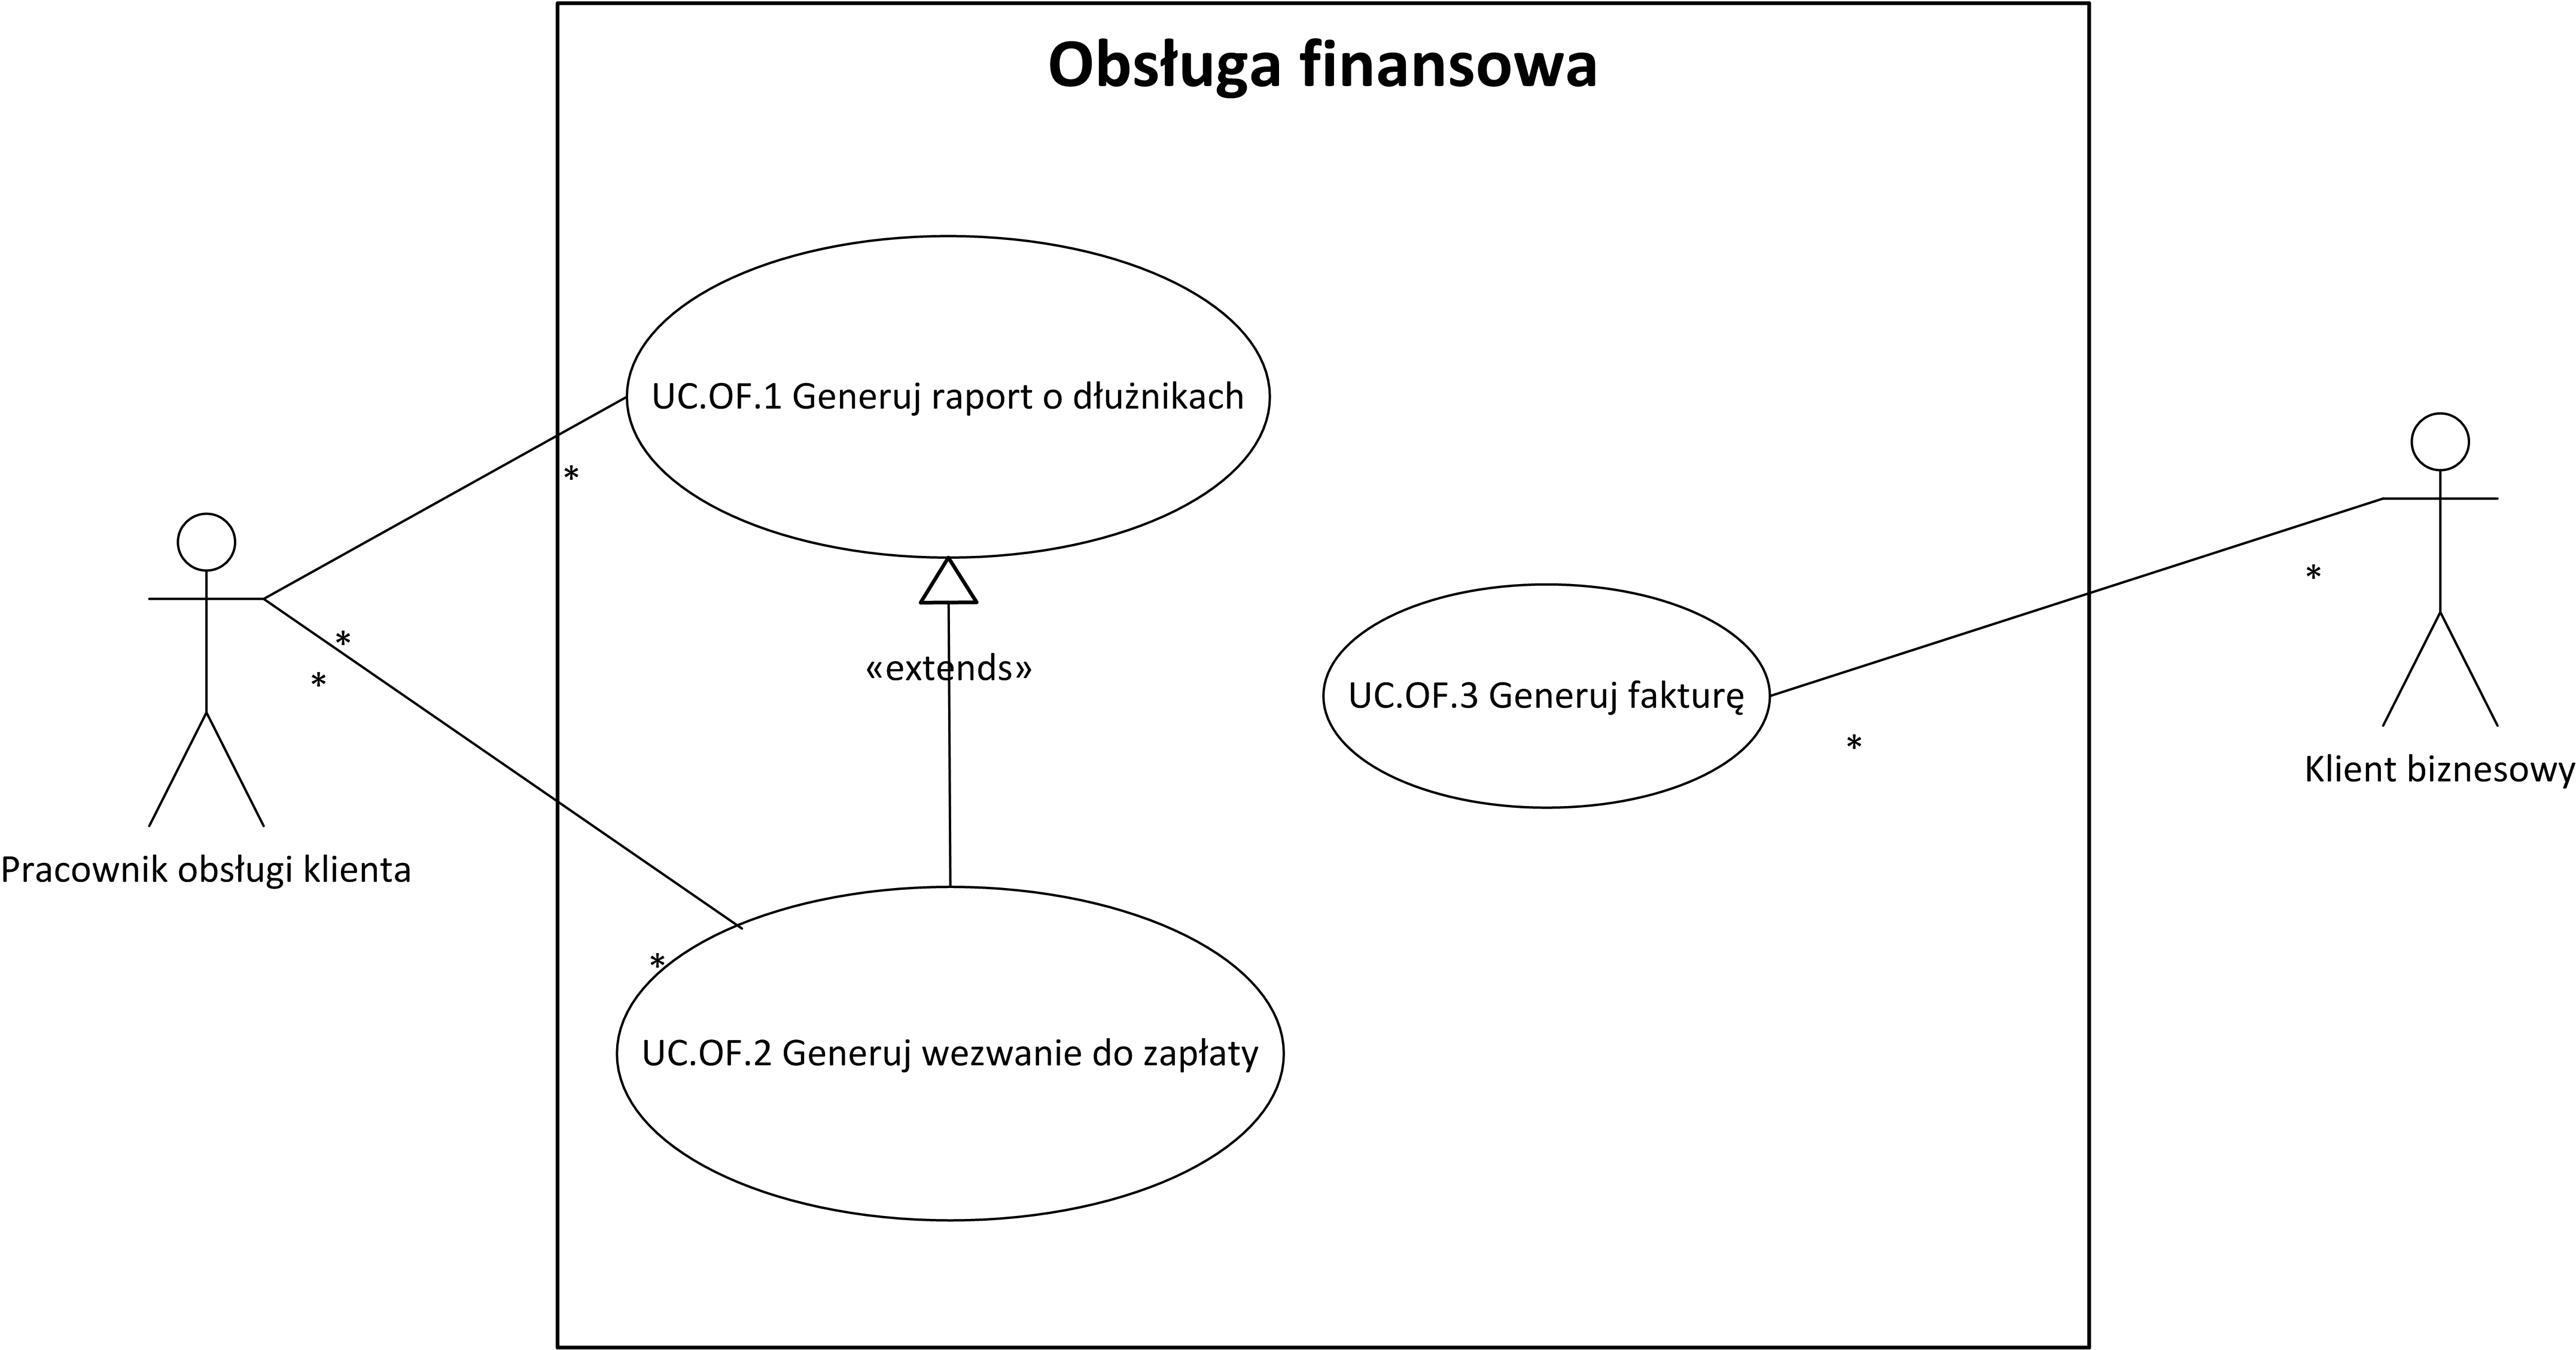
\includegraphics[width=\textwidth]{img/obs_fin_uc}
\end{figure}

\subsubsection*{Scenariusze przypadków użycia}
\begin{center}
\begin{longtable}[h]{|p{1.6cm}|p{13.5cm}|}
\hline
\textbf{ID:} & UC.OF.1 \\ \hline
\textbf{Nazwa:} & Generuj raport o dłużnikach \\ \hline
\multicolumn{2}{|p{15.1cm}|}{\textbf{Aktorzy główni:} Pracownik obsługi klienta} \\
\multicolumn{2}{|p{15.1cm}|}{\textbf{Aktorzy pomocniczy:} 
\textit{brak}} \\
\multicolumn{2}{|p{15.1cm}|}{\textbf{Poziom:} Użytkownika} \\
\multicolumn{2}{|p{15.1cm}|}{\textbf{Priorytet:} Średni} \\
\hline
\multicolumn{2}{|p{15.1cm}|}{\textbf{Opis:}} \\
\multicolumn{2}{|p{15.1cm}|}{
Pracownik chce wygenerować raport o klient zalegających z płatnościami za usługi.
} \\ \hline
\multicolumn{2}{|p{15.1cm}|}{\textbf{Wyzwalacze:}} \\
\multicolumn{2}{|p{15.1cm}|}{
Aktor wybiera opcję ''Generuj raport o dłużnikach'' w aplikacji klienckiej.
} \\ \hline
\multicolumn{2}{|p{15.1cm}|}{\textbf{Warunki początkowe:}} \\
\multicolumn{2}{|p{15.1cm}|}{
Aktor jest zalogowany w aplikacji klienckiej.
} \\ \hline
\multicolumn{2}{|p{15.1cm}|}{\textbf{Warunki końcowe:}} \\
\multicolumn{2}{|p{15.1cm}|}{
Raport o dłużnikach zostaje zaprezentowany aktorowi.
} \\ \hline
\multicolumn{2}{|p{15.1cm}|}{\textbf{Scenariusz główny:}} \\
\multicolumn{2}{|p{15.1cm}|}{
\begin{enumerate}
\item Aktor wybiera opcję ''Generuj raport o dłużnikach'' w aplikacji klienckiej.
\item System pobiera listę dostępnych klientów biznesowych.
\item System prezentuje listę klientów biznesowych.
\item Aktor zaznacza klientów o których chce sporządzić raport.
\item System generuje raporty zadłużenia dla zaznaczonych klientów.
\item System zapisuje raporty w aplikacji.
\item System umożliwia otwarcie wygenerowanych raportów.
\end{enumerate}
} \\ \hline
\multicolumn{2}{|p{15.1cm}|}{\textbf{Scenariusze alternatywne i rozszerzenia:}} \\
\multicolumn{2}{|p{15.1cm}|}{
4.a Aktor nie wybrał żadnego klienta. \newline
4.a.1 System prezentuje ostrzeżenie o nie wybraniu żadnego klienta. \newline
4.a.2 Aktor koryguje listę wybranych klientów. \newline
4.a.3 Powrót do punktu 5 scenariusza głównego.
} \\ \hline
\multicolumn{2}{|p{15.1cm}|}{\textbf{Wyjątki:}} \\
\multicolumn{2}{|p{15.1cm}|}{
\textit{brak}
} \\ \hline
\multicolumn{2}{|p{15.1cm}|}{\textbf{Dodatkowe wymagania:}} \\
\multicolumn{2}{|p{15.1cm}|}{
\textit{brak}
} \\
\hline
\end{longtable}
\end{center}

\begin{center}
\begin{longtable}[h]{|p{1.6cm}|p{13.5cm}|}
\hline
\textbf{ID:} & UC.OF.2 \\ \hline
\textbf{Nazwa:} & Generuj wezwanie do zapłaty \\ \hline
\multicolumn{2}{|p{15.1cm}|}{\textbf{Aktorzy główni:} Pracownik obsługi klienta} \\
\multicolumn{2}{|p{15.1cm}|}{\textbf{Aktorzy pomocniczy:} 
\textit{brak}} \\
\multicolumn{2}{|p{15.1cm}|}{\textbf{Poziom:} Użytkownika} \\
\multicolumn{2}{|p{15.1cm}|}{\textbf{Priorytet:} Średni} \\
\hline
\multicolumn{2}{|p{15.1cm}|}{\textbf{Opis:}} \\
\multicolumn{2}{|p{15.1cm}|}{
Aktor chce wygenerować wezwanie do zapłaty dla klienta biznesowego, który zalega z płatnościami za usługi.
} \\ \hline
\multicolumn{2}{|p{15.1cm}|}{\textbf{Wyzwalacze:}} \\
\multicolumn{2}{|p{15.1cm}|}{
Aktor wygenerował Raporty o zadłużeniach i wybrał opcję ''Utwórz wezwanie do zapłaty'' obok jednego z raportów.
} \\ \hline
\multicolumn{2}{|p{15.1cm}|}{\textbf{Warunki początkowe:}} \\
\multicolumn{2}{|p{15.1cm}|}{
1. Aktor jest zalogowany do aplikacji klienckiej. \newline
2. Aktor wygenerował listę raportów o zadłużeniach.
} \\ \hline
\multicolumn{2}{|p{15.1cm}|}{\textbf{Warunki końcowe:}} \\
\multicolumn{2}{|p{15.1cm}|}{
Wezwanie do zapłaty zostaje wygenerowane i system umożliwia jego wydruk.
} \\ \hline
\multicolumn{2}{|p{15.1cm}|}{\textbf{Scenariusz główny:}} \\
\multicolumn{2}{|p{15.1cm}|}{
\begin{enumerate}
\item Aktor wybiera opcję ''Utwórz wezwanie do zapłaty'' obok jednego z raportów o zadłużeniach.
\item System prezentuje listę pozycji które składają się na raport.
\item Aktor wybiera pozycje dla których chce wygenerować wezwanie.
\item System generuje wezwanie do zapłaty dla wskazanego klienta biznesowego oraz wybranych pozycji.
\item System prezentuje wygenerowane wezwanie do zapłaty.
\item Aktor wybiera opcję ''Drukuj raport'' w celu wydrukowania raportu.
\item System przesyła żądanie wydruku do drukarki.
\end{enumerate}
} \\ \hline
\multicolumn{2}{|p{15.1cm}|}{\textbf{Scenariusze alternatywne i rozszerzenia:}} \\
\multicolumn{2}{|p{15.1cm}|}{
3.a Aktor nie wybrał żadnej pozycji zadłużenia. \newline
3.a.1 System prezentuje ostrzeżenie. \newline
3.a.2 Aktor poprawia wybór pozycji. \newline
3.a.3 Powrót do punktu 4 scenariusza głównego. \newline
\newline
6.a Aplikacja kliencka nie ma połączenia z drukarką. \newline
6.a.1 System blokuje przycisk ''Drukuj raport''. \newline
6.a.2 Przypadek użycia kończy się. \newline
} \\ \hline
\multicolumn{2}{|p{15.1cm}|}{\textbf{Wyjątki:}} \\
\multicolumn{2}{|p{15.1cm}|}{
\textit{brak}} \\ \hline
\multicolumn{2}{|p{15.1cm}|}{\textbf{Dodatkowe wymagania:}} \\
\multicolumn{2}{|p{15.1cm}|}{
Dostęp aplikacji klienckiej do drukarki.
} \\
\hline
\end{longtable}
\end{center}

\begin{center}
\begin{longtable}[h]{|p{1.6cm}|p{13.5cm}|}
\hline
\textbf{ID:} & UC.OF.3 \\ \hline
\textbf{Nazwa:} & Generuj fakturę \\ \hline
\multicolumn{2}{|p{15.1cm}|}{\textbf{Aktorzy główni:} Klient biznesowy} \\
\multicolumn{2}{|p{15.1cm}|}{\textbf{Aktorzy pomocniczy:} 
\textit{brak}} \\
\multicolumn{2}{|p{15.1cm}|}{\textbf{Poziom:} Użytkownika} \\
\multicolumn{2}{|p{15.1cm}|}{\textbf{Priorytet:} Wysoki} \\
\hline
\multicolumn{2}{|p{15.1cm}|}{\textbf{Opis:}} \\
\multicolumn{2}{|p{15.1cm}|}{
Klient biznesowy chce wygenerować fakturę za wybrane usługi.
} \\ \hline
\multicolumn{2}{|p{15.1cm}|}{\textbf{Wyzwalacze:}} \\
\multicolumn{2}{|p{15.1cm}|}{
Aktor wybiera opcję ''Generuj fakturę'' w interfejsie internetowym.
} \\ \hline
\multicolumn{2}{|p{15.1cm}|}{\textbf{Warunki początkowe:}} \\
\multicolumn{2}{|p{15.1cm}|}{
Aktor jest zalogowany w interfejsie internetowym.
} \\ \hline
\multicolumn{2}{|p{15.1cm}|}{\textbf{Warunki końcowe:}} \\
\multicolumn{2}{|p{15.1cm}|}{
Faktura zostaje wygenerowana i system umożliwia pobrania jej w formacie PDF.
} \\ \hline
\multicolumn{2}{|p{15.1cm}|}{\textbf{Scenariusz główny:}} \\
\multicolumn{2}{|p{15.1cm}|}{
\begin{enumerate}
\item Aktor wybiera opcję ''Generuj fakturę''.
\item System prezentuje listę nieopłaconych usług klienta.
\item Aktor wybiera usługi za które chce uzyskać fakturę.
\item System generuje fakturę na podstawie wskazanych pozycji.
\item System prezentuje wygenerowaną fakturę.
\item System umożliwia pobranie faktury w formie pliku PDF.
\end{enumerate}
} \\ \hline
\multicolumn{2}{|p{15.1cm}|}{\textbf{Scenariusze alternatywne i rozszerzenia:}} \\
\multicolumn{2}{|p{15.1cm}|}{
3.a Aktor nie wskazał żadnej pozycji. \newline
3.a.1 System prezentuje ostrzeżenie. \newline
3.a.2 Aktor koryguje swój wybór. \newline
3.a.3 Powrót do punktu 4 scenariusza głównego. 
} \\ \hline
\multicolumn{2}{|p{15.1cm}|}{\textbf{Wyjątki:}} \\
\multicolumn{2}{|p{15.1cm}|}{
\textit{brak}
} \\ \hline
\multicolumn{2}{|p{15.1cm}|}{\textbf{Dodatkowe wymagania:}} \\
\multicolumn{2}{|p{15.1cm}|}{
\textit{brak}
} \\
\hline
\end{longtable}
\end{center}

\subsection{Moduł informacyjny i obsługi klienta}
\subsubsection*{Opis}
Moduł zawiera funkcjonalności dostarczające informację klientowi informację o usługach Firmy Kurierskiej. Zawiera również opis funkcjonalności logowania do systemu oraz obsługę reklamacji. Definiuje także funkcję nadania przesyłki w POK.

\subsubsection*{Przypadki użycia}
\begin{figure}[H]
\centering
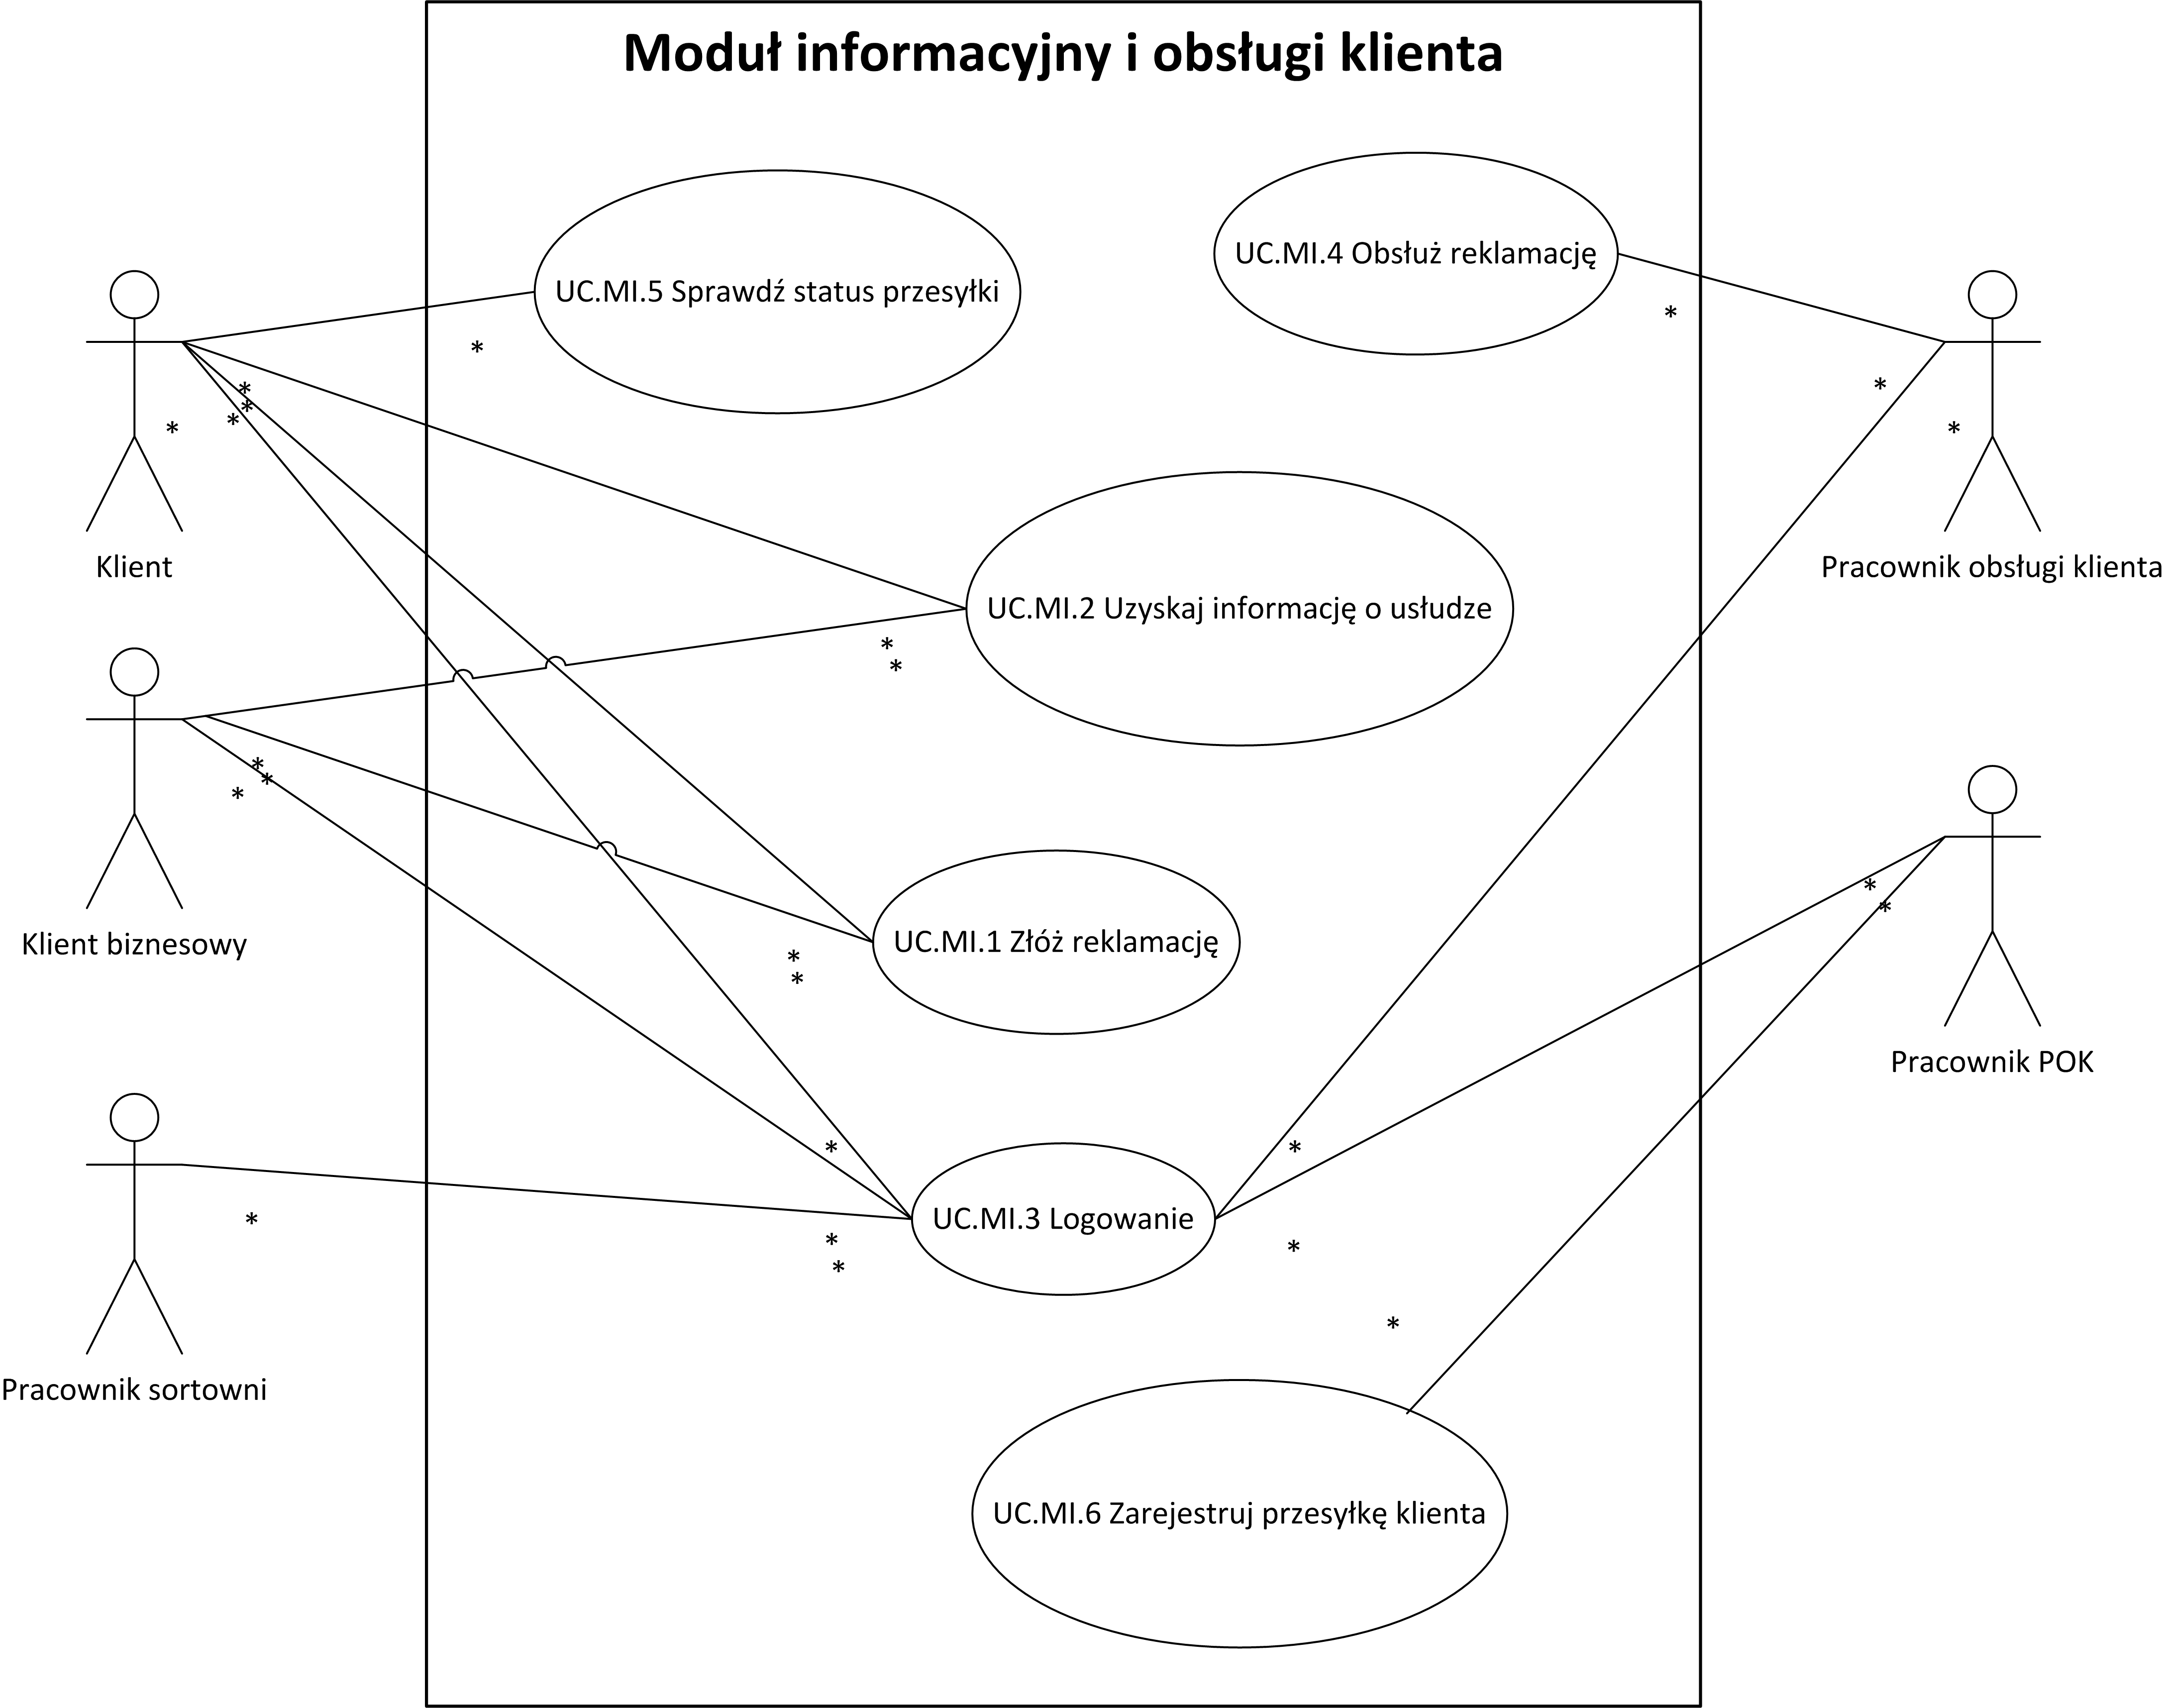
\includegraphics[width=\textwidth]{img/mod_inf_uc}
\end{figure}

\subsubsection*{Scenariusze przypadków użycia}
\begin{center}
\begin{longtable}[h]{|p{1.6cm}|p{13.5cm}|}
\hline
\textbf{ID:} & UC.MI.1 \\ \hline
\textbf{Nazwa:} & Złóż reklamację \\ \hline
\multicolumn{2}{|p{15.1cm}|}{\textbf{Aktorzy główni:} Klient lub Klient biznesowy} \\
\multicolumn{2}{|p{15.1cm}|}{\textbf{Aktorzy pomocniczy:}
\textit{brak}} \\
\multicolumn{2}{|p{15.1cm}|}{\textbf{Poziom:} Użytkownika} \\
\multicolumn{2}{|p{15.1cm}|}{\textbf{Priorytet:} Wysoki} \\
\hline
\multicolumn{2}{|p{15.1cm}|}{\textbf{Opis:}} \\
\multicolumn{2}{|p{15.1cm}|}{
Klient lub Klient biznesowy chce złożyć reklamację na wykonanie usługi.
} \\ \hline
\multicolumn{2}{|p{15.1cm}|}{\textbf{Wyzwalacze:}} \\
\multicolumn{2}{|p{15.1cm}|}{
Aktor wybiera opcję ''Złóż reklamację'' w interfejsie internetowym.
} \\ \hline
\multicolumn{2}{|p{15.1cm}|}{\textbf{Warunki początkowe:}} \\
\multicolumn{2}{|p{15.1cm}|}{
Aktor jest zalogowany w interfejsie internetowym.
} \\ \hline
\multicolumn{2}{|p{15.1cm}|}{\textbf{Warunki końcowe:}} \\
\multicolumn{2}{|p{15.1cm}|}{
Reklamacja zostaje zarejestrowana w systemie.
} \\ \hline
\multicolumn{2}{|p{15.1cm}|}{\textbf{Scenariusz główny:}} \\
\multicolumn{2}{|p{15.1cm}|}{
\begin{enumerate}
\item Aktor wybiera opcję ''Złóż reklamację''.
\item System prezentuje formularz reklamacji.
\item System uzupełnia dane klienta w formularzu na podstawie danych konta.
\item Aktor wprowadza numery przesyłek których dotyczy reklamacja.
\item Aktor wprowadza opis reklamacji.
\item System sprawdza poprawność wprowadzonych danych.
\item System nadaje reklamacji identyfikator i zapisuje ją w systemie.
\item System wyświetla potwierdzenie złożenia reklamacji.
\end{enumerate}
} \\ \hline
\multicolumn{2}{|p{15.1cm}|}{\textbf{Scenariusze alternatywne i rozszerzenia:}} \\
\multicolumn{2}{|p{15.1cm}|}{
6.a Wprowadzone dane są niepoprawne. \newline
6.a.1 System wyświetla informacje o błędnych danych. \newline
6.a.2 Aktor poprawia wprowadzone dane. \newline
6.a.3 Powrót do punktu 6 scenariusza głównego.
} \\ \hline
\multicolumn{2}{|p{15.1cm}|}{\textbf{Wyjątki:}} \\
\multicolumn{2}{|p{15.1cm}|}{
\textit{brak}
} \\ \hline
\multicolumn{2}{|p{15.1cm}|}{\textbf{Dodatkowe wymagania:}} \\
\multicolumn{2}{|p{15.1cm}|}{
\textit{brak}
} \\
\hline
\end{longtable}
\end{center}

\begin{center}
\begin{longtable}[h]{|p{1.6cm}|p{13.5cm}|}
\hline
\textbf{ID:} & UC.MI.2 \\ \hline
\textbf{Nazwa:} & Uzyskaj informacje o usłudze \\ \hline
\multicolumn{2}{|p{15.1cm}|}{\textbf{Aktorzy główni:} Klient lub Klient biznesowy} \\
\multicolumn{2}{|p{15.1cm}|}{\textbf{Aktorzy pomocniczy:} 
\textit{brak}} \\
\multicolumn{2}{|p{15.1cm}|}{\textbf{Poziom:} Użytkownika} \\
\multicolumn{2}{|p{15.1cm}|}{\textbf{Priorytet:} Wysoki} \\
\hline
\multicolumn{2}{|p{15.1cm}|}{\textbf{Opis:}} \\
\multicolumn{2}{|p{15.1cm}|}{
Aktor chce uzyskać informację o usłudze dostarczanej przez Firmę Kurierską.
} \\ \hline
\multicolumn{2}{|p{15.1cm}|}{\textbf{Wyzwalacze:}} \\
\multicolumn{2}{|p{15.1cm}|}{
Aktor przechodzi do menu ''Informacje'' interfejsu internetowego.
} \\ \hline
\multicolumn{2}{|p{15.1cm}|}{\textbf{Warunki początkowe:}} \\
\multicolumn{2}{|p{15.1cm}|}{
\textit{brak}
} \\ \hline
\multicolumn{2}{|p{15.1cm}|}{\textbf{Warunki końcowe:}} \\
\multicolumn{2}{|p{15.1cm}|}{
System prezentuje informacje o wybranej usłudze.
} \\ \hline
\multicolumn{2}{|p{15.1cm}|}{\textbf{Scenariusz główny:}} \\
\multicolumn{2}{|p{15.1cm}|}{
\begin{enumerate}
\item Aktor przechodzi do menu ''Informacje''.
\item System prezentuje listę dostępnych usług.
\item Aktor wskazuje wybraną usługę.
\item System prezentuje informacje o wybranej usłudze.
\end{enumerate}
} \\ \hline
\multicolumn{2}{|p{15.1cm}|}{\textbf{Scenariusze alternatywne i rozszerzenia:}} \\
\multicolumn{2}{|p{15.1cm}|}{
\textit{brak}} \\ \hline
\multicolumn{2}{|p{15.1cm}|}{\textbf{Wyjątki:}} \\
\multicolumn{2}{|p{15.1cm}|}{
\textit{brak}
} \\ \hline
\multicolumn{2}{|p{15.1cm}|}{\textbf{Dodatkowe wymagania:}} \\
\multicolumn{2}{|p{15.1cm}|}{
\textit{brak}
} \\
\hline
\end{longtable}
\end{center}

\begin{center}
\begin{longtable}[h]{|p{1.6cm}|p{13.5cm}|}
\hline
\textbf{ID:} & UC.MI.3 \\ \hline
\textbf{Nazwa:} & Logowanie \\ \hline
\multicolumn{2}{|p{15.1cm}|}{\textbf{Aktorzy główni:} Klient lub Klient biznesowy lub Pracownik sortowni lub Pracownik obsługi klienta lub Pracownik POK} \\
\multicolumn{2}{|p{15.1cm}|}{\textbf{Aktorzy pomocniczy:} 
\textit{brak}} \\
\multicolumn{2}{|p{15.1cm}|}{\textbf{Poziom:} Użytkownika} \\
\multicolumn{2}{|p{15.1cm}|}{\textbf{Priorytet:} Wysoki} \\
\hline
\multicolumn{2}{|p{15.1cm}|}{\textbf{Opis:}} \\
\multicolumn{2}{|p{15.1cm}|}{
Aktor chce się zalogować do jednego z interfejsów SWPFK.
} \\ \hline
\multicolumn{2}{|p{15.1cm}|}{\textbf{Wyzwalacze:}} \\
\multicolumn{2}{|p{15.1cm}|}{
Wybranie opcji ''Zaloguje'' w jednym z interfejsów SWPFK.
} \\ \hline
\multicolumn{2}{|p{15.1cm}|}{\textbf{Warunki początkowe:}} \\
\multicolumn{2}{|p{15.1cm}|}{
Aktor posiada dane do logowania w systemie.
} \\ \hline
\multicolumn{2}{|p{15.1cm}|}{\textbf{Warunki końcowe:}} \\
\multicolumn{2}{|p{15.1cm}|}{
Aktor zostaje zalogowany oraz zostaje utworzona nowa sesja w systemie.
} \\ \hline
\multicolumn{2}{|p{15.1cm}|}{\textbf{Scenariusz główny:}} \\
\multicolumn{2}{|p{15.1cm}|}{
\begin{enumerate}
\item Aktor wybiera opcję ''Zaloguj''.
\item System prezentuje formularz logowania.
\item Aktor wprowadza Identyfikator oraz Hasło.
\item System sprawdza poprawność danych.
\item System loguje użytkownika w systemie.
\item System prezentuje informacje o pomyślnym zalogowaniu.
\end{enumerate}
} \\ \hline
\multicolumn{2}{|p{15.1cm}|}{\textbf{Scenariusze alternatywne i rozszerzenia:}} \\
\multicolumn{2}{|p{15.1cm}|}{
4.a Wprowadzone dane są niepoprawne. \newline
4.a.1 System prezentuje informacje o niepoprawnych danych logowania. \newline
4.a.2 Aktor poprawia wprowadzone dane. \newline
4.a.3 Powrót do punktu 4 scenariusza głównego.
} \\ \hline
\multicolumn{2}{|p{15.1cm}|}{\textbf{Wyjątki:}} \\
\multicolumn{2}{|p{15.1cm}|}{
\textit{brak}
} \\ \hline
\multicolumn{2}{|p{15.1cm}|}{\textbf{Dodatkowe wymagania:}} \\
\multicolumn{2}{|p{15.1cm}|}{
\textit{brak}
} \\
\hline
\end{longtable}
\end{center}

\begin{center}
\begin{longtable}[h]{|p{1.6cm}|p{13.5cm}|}
\hline
\textbf{ID:} & UC.MI.4 \\ \hline
\textbf{Nazwa:} & Obsłuż reklamację \\ \hline
\multicolumn{2}{|p{15.1cm}|}{\textbf{Aktorzy główni:} ID lub nazwy aktorów głównych biorących udział w procesie} \\
\multicolumn{2}{|p{15.1cm}|}{\textbf{Aktorzy pomocniczy:} ID lub nazwy aktorów pomocniczych biorących udział w procesie} \\
\multicolumn{2}{|p{15.1cm}|}{\textbf{Poziom:}  Biznesowy / Użytkownika / Podfunkcji} \\
\multicolumn{2}{|p{15.1cm}|}{\textbf{Priorytet:}  Niski / Średni / Wysoki} \\
\hline
\multicolumn{2}{|p{15.1cm}|}{\textbf{Opis:}} \\
\multicolumn{2}{|p{15.1cm}|}{Opis procesu biznesowego.
} \\ \hline
\multicolumn{2}{|p{15.1cm}|}{\textbf{Wyzwalacze:}} \\
\multicolumn{2}{|p{15.1cm}|}{Wyszczególnienie zdarzeń wyzwalających proces.
} \\ \hline
\multicolumn{2}{|p{15.1cm}|}{\textbf{Warunki początkowe:}} \\
\multicolumn{2}{|p{15.1cm}|}{Warunki początkowe procesu.
} \\ \hline
\multicolumn{2}{|p{15.1cm}|}{\textbf{Warunki końcowe:}} \\
\multicolumn{2}{|p{15.1cm}|}{Warunki końcowe procesu.
} \\ \hline
\multicolumn{2}{|p{15.1cm}|}{\textbf{Scenariusz główny:}} \\
\multicolumn{2}{|p{15.1cm}|}{Scenariusz główny procesu.
} \\ \hline
\multicolumn{2}{|p{15.1cm}|}{\textbf{Scenariusze alternatywne i rozszerzenia:}} \\
\multicolumn{2}{|p{15.1cm}|}{Scenariusze alternatywne procesu.
} \\ \hline
\multicolumn{2}{|p{15.1cm}|}{\textbf{Wyjątki:}} \\
\multicolumn{2}{|p{15.1cm}|}{Wyjątki procesu.
} \\ \hline
\multicolumn{2}{|p{15.1cm}|}{\textbf{Dodatkowe wymagania:}} \\
\multicolumn{2}{|p{15.1cm}|}{Dodatkowe wymagania procesu.
} \\
\hline
\end{longtable}
\end{center}

\begin{center}
\begin{longtable}[h]{|p{1.6cm}|p{13.5cm}|}
\hline
\textbf{ID:} & UC.MI.5 \\ \hline
\textbf{Nazwa:} & Sprawdź status przesyłki \\ \hline
\multicolumn{2}{|p{15.1cm}|}{\textbf{Aktorzy główni:} Klient} \\
\multicolumn{2}{|p{15.1cm}|}{\textbf{Aktorzy pomocniczy:} 
\textit{brak}} \\
\multicolumn{2}{|p{15.1cm}|}{\textbf{Poziom:} Użytkownika} \\
\multicolumn{2}{|p{15.1cm}|}{\textbf{Priorytet:} Średni} \\
\hline
\multicolumn{2}{|p{15.1cm}|}{\textbf{Opis:}} \\
\multicolumn{2}{|p{15.1cm}|}{
Klient chce sprawdzić status przesyłki.
} \\ \hline
\multicolumn{2}{|p{15.1cm}|}{\textbf{Wyzwalacze:}} \\
\multicolumn{2}{|p{15.1cm}|}{
Aktor wybiera opcję ''Sprawdź status przesyłki'' w interfejsie internetowym.
} \\ \hline
\multicolumn{2}{|p{15.1cm}|}{\textbf{Warunki początkowe:}} \\
\multicolumn{2}{|p{15.1cm}|}{
Aktor posiada numer przesyłki, której status chce sprawdzić.
} \\ \hline
\multicolumn{2}{|p{15.1cm}|}{\textbf{Warunki końcowe:}} \\
\multicolumn{2}{|p{15.1cm}|}{
System prezentuje status przesyłki.
} \\ \hline
\multicolumn{2}{|p{15.1cm}|}{\textbf{Scenariusz główny:}} \\
\multicolumn{2}{|p{15.1cm}|}{
\begin{enumerate}
\item Aktor wybiera opcję ''Sprawdź status przesyłki''.
\item System prezentuje formularz do wprowadzenia numeru przesyłki.
\item Aktor wprowadza numer przesyłki.
\item System wyszukuje status przesyłki o podanym numerze.
\item System prezentuje status przesyłki.
\end{enumerate}
} \\ \hline
\multicolumn{2}{|p{15.1cm}|}{\textbf{Scenariusze alternatywne i rozszerzenia:}} \\
\multicolumn{2}{|p{15.1cm}|}{
4.a Wprowadzony numer przesyłki jest niepoprawny. \newline
4.a.1 System prezentuje informacje o niepoprawnym numerze przesyłki. \newline
4.a.2 Aktor ponownie wprowadza numer przesyłki. \newline
4.a.3 Powrót do punktu 4 scenariusza głównego. \newline
} \\ \hline
\multicolumn{2}{|p{15.1cm}|}{\textbf{Wyjątki:}} \\
\multicolumn{2}{|p{15.1cm}|}{
\textit{brak}
} \\ \hline
\multicolumn{2}{|p{15.1cm}|}{\textbf{Dodatkowe wymagania:}} \\
\multicolumn{2}{|p{15.1cm}|}{
\textit{brak}
} \\
\hline
\end{longtable}
\end{center}

\begin{center}
\begin{longtable}[h]{|p{1.6cm}|p{13.5cm}|}
\hline
\textbf{ID:} & UC.MI.6 \\ \hline
\textbf{Nazwa:} & Zarejestruj przesyłkę klienta \\ \hline
\multicolumn{2}{|p{15.1cm}|}{\textbf{Aktorzy główni:} Pracownik POK} \\
\multicolumn{2}{|p{15.1cm}|}{\textbf{Aktorzy pomocniczy:} Klient} \\
\multicolumn{2}{|p{15.1cm}|}{\textbf{Poziom:} Użytkownika} \\
\multicolumn{2}{|p{15.1cm}|}{\textbf{Priorytet:} Średni} \\
\hline
\multicolumn{2}{|p{15.1cm}|}{\textbf{Opis:}} \\
\multicolumn{2}{|p{15.1cm}|}{
Pracownik POK chce zarejestrować przesyłkę przyniesioną przez Klienta.
} \\ \hline
\multicolumn{2}{|p{15.1cm}|}{\textbf{Wyzwalacze:}} \\
\multicolumn{2}{|p{15.1cm}|}{
Klient przychodzi do POK w celu wysłania przesyłki.
} \\ \hline
\multicolumn{2}{|p{15.1cm}|}{\textbf{Warunki początkowe:}} \\
\multicolumn{2}{|p{15.1cm}|}{
Aktor jest zalogowany w aplikacji klienckiej.
} \\ \hline
\multicolumn{2}{|p{15.1cm}|}{\textbf{Warunki końcowe:}} \\
\multicolumn{2}{|p{15.1cm}|}{
Przesyłka zostaje zarejestrowana w systemie i zostaje jej nadany numer.
} \\ \hline
\multicolumn{2}{|p{15.1cm}|}{\textbf{Scenariusz główny:}} \\
\multicolumn{2}{|p{15.1cm}|}{
\begin{enumerate}
\item Aktor wybiera opcję ''Zarejestruj przesyłkę'' w menu aplikacji klienckiej.
\item System prezentuje formularz rejestrowania przesyłki.
\item Aktor wprowadza dane nadawcy oraz odbiorcy.
\item Aktor wprowadza parametry przesyłki, takie jak wymiary i waga.
\item Aplikacja kliencka przesyła do modułu serwerowego żądanie zarejestrowania przesyłki.
\item Moduł serwerowy nadaje przesyłce unikalny numer oraz rejestruje ją w systemie.
\item Moduł serwerowy przesyła potwierdzenie zarejestrowania przesyłki.
\item Aplikacja kliencka prezentuje potwierdzenie zarejestrowania.
\item Aktor wybiera opcję ''Drukuj potwierdzenie''.
\item Aplikacja kliencka przesyła żądanie drukowania do drukarki.
\end{enumerate}
} \\ \hline
\multicolumn{2}{|p{15.1cm}|}{\textbf{Scenariusze alternatywne i rozszerzenia:}} \\
\multicolumn{2}{|p{15.1cm}|}{

} \\ \hline
\multicolumn{2}{|p{15.1cm}|}{\textbf{Wyjątki:}} \\
\multicolumn{2}{|p{15.1cm}|}{
Aplikacja kliencka nie ma połączenia z modułem serwerowym.
} \\ \hline
\multicolumn{2}{|p{15.1cm}|}{\textbf{Dodatkowe wymagania:}} \\
\multicolumn{2}{|p{15.1cm}|}{
Aplikacja kliencka ma dostęp do drukarki.
} \\
\hline
\end{longtable}
\end{center}

\subsection{Obsługa doręczeń i odbiorów}
\subsubsection*{Opis}
Moduł zawiera funkcjonalności związane z bezpośrednim doręczeniem i odbiorem przesyłek od klienta.

\subsubsection*{Przypadki użycia}
\begin{figure}[H]
\centering
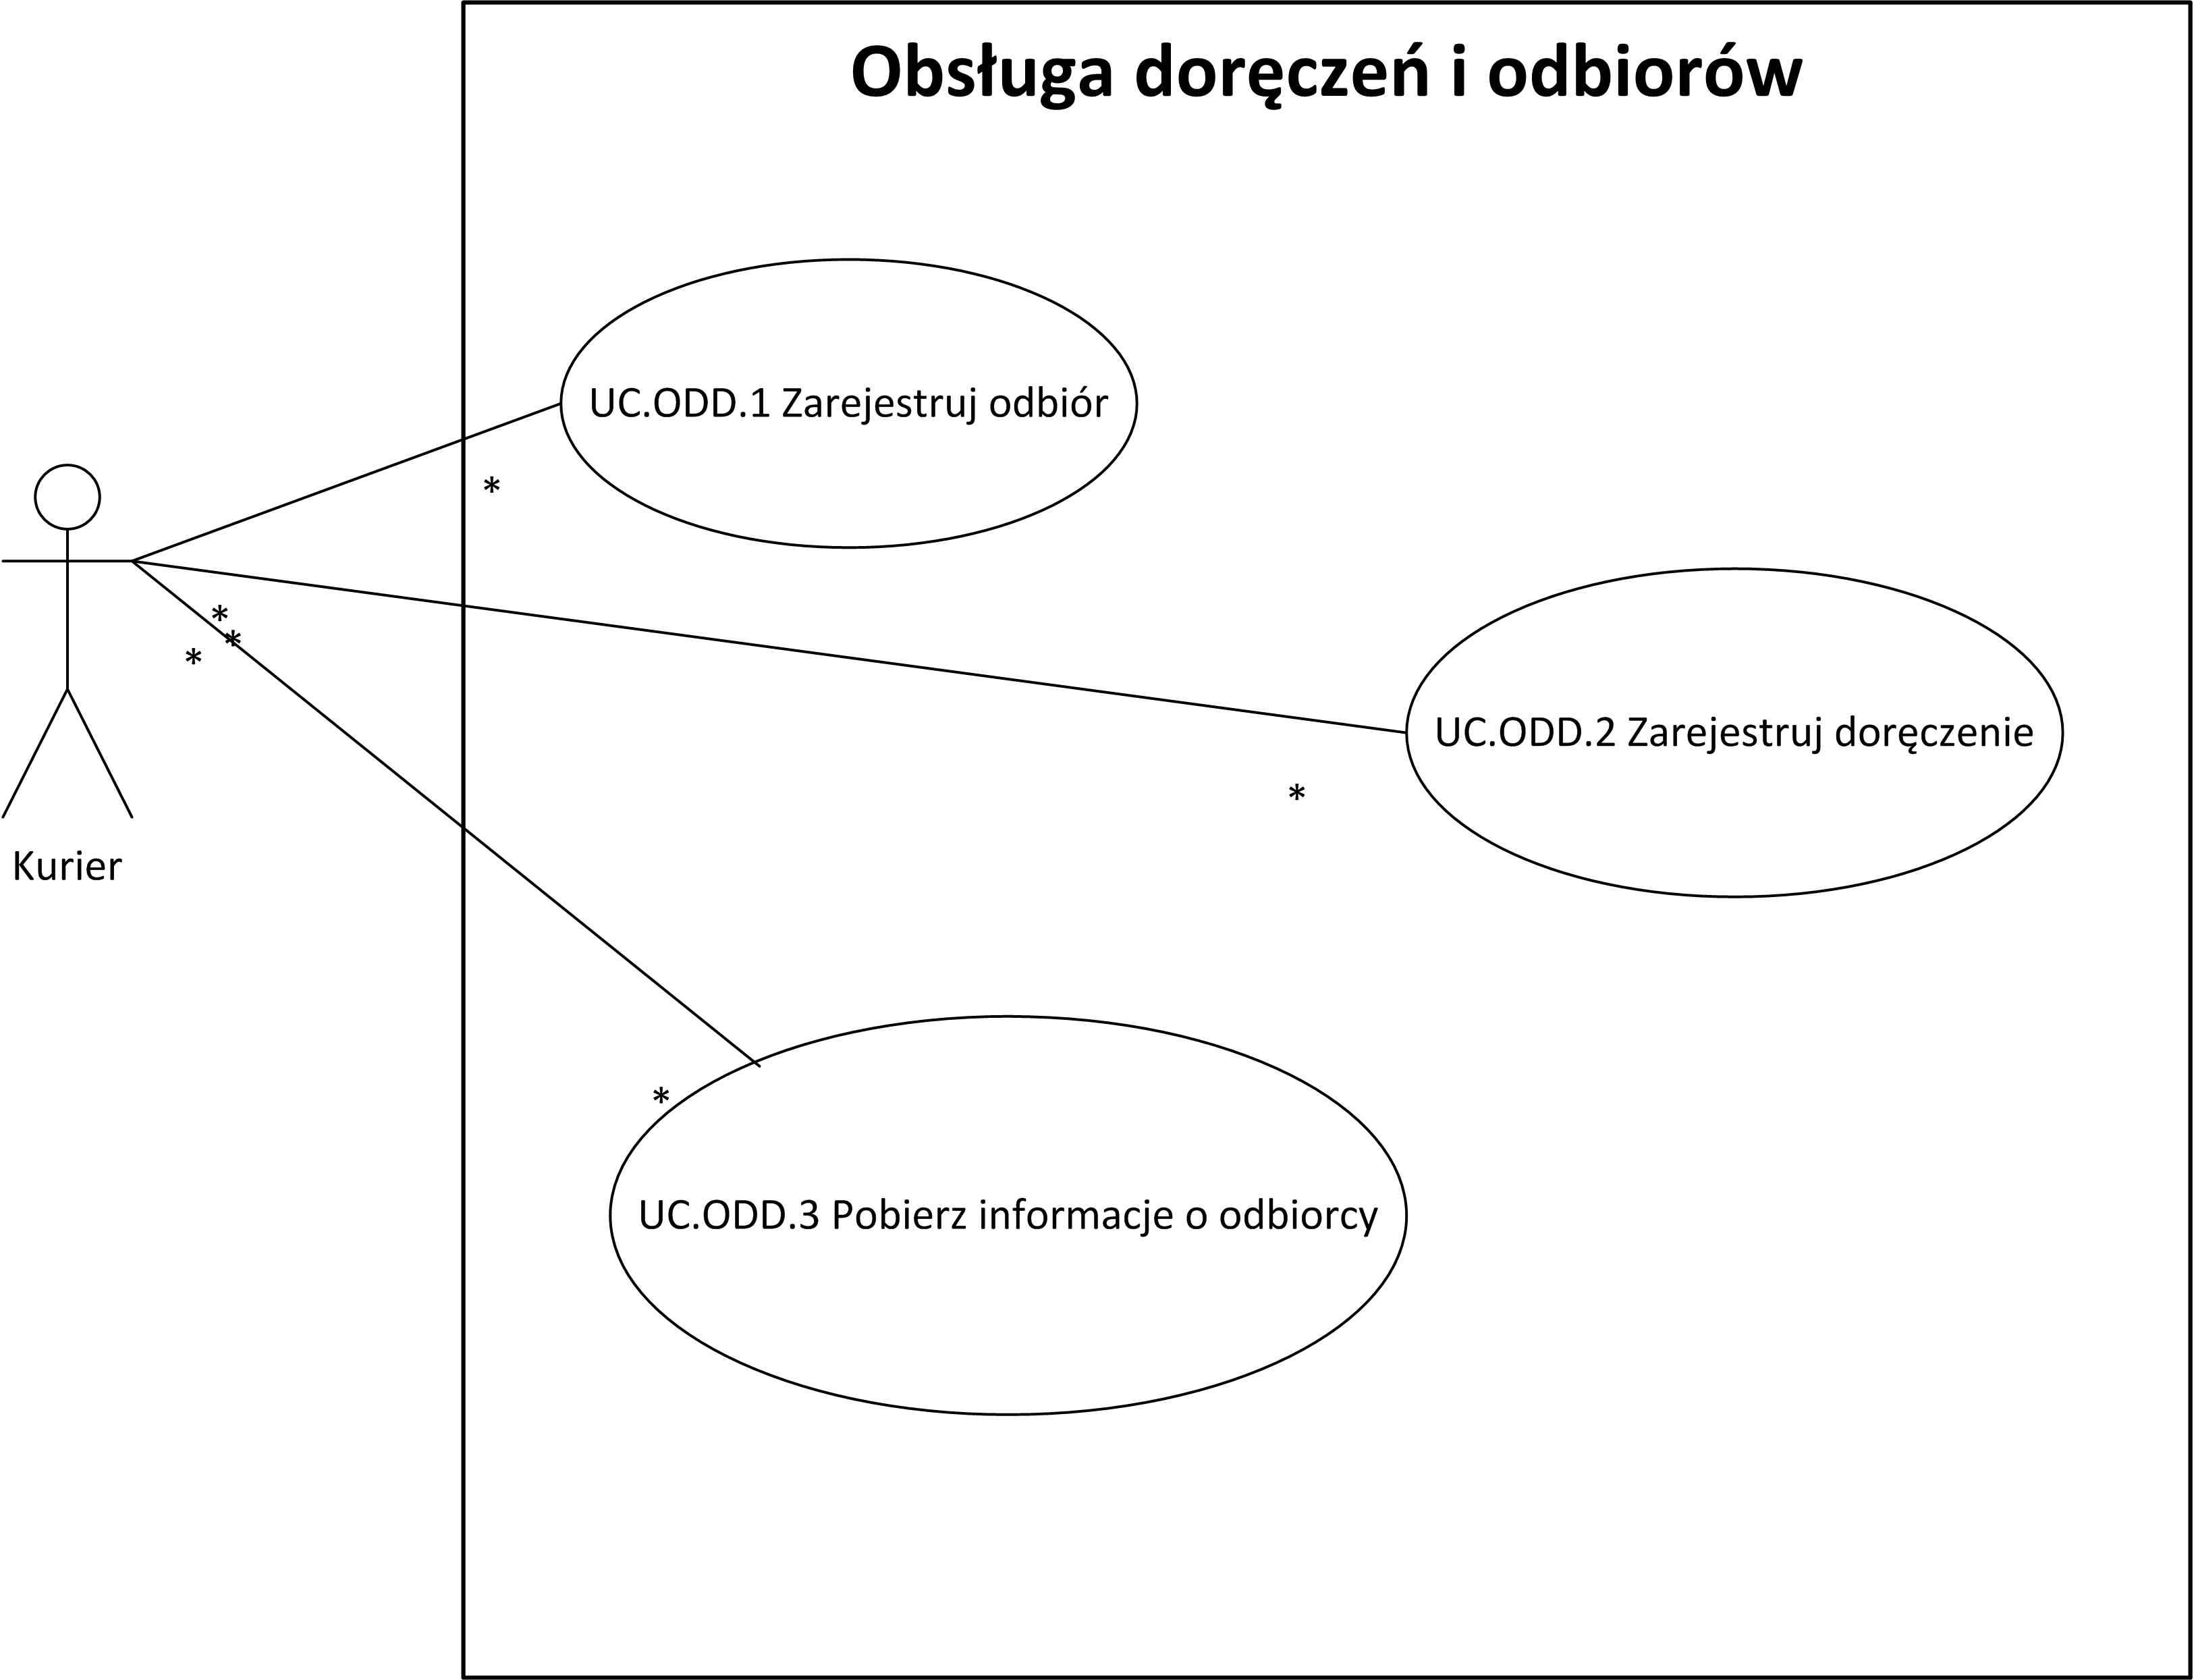
\includegraphics[width=\textwidth]{img/obs_dor_odb_uc}
\end{figure}

\subsubsection*{Scenariusze przypadków użycia}
\begin{center}
\begin{longtable}[h]{|p{1.6cm}|p{13.5cm}|}
\hline
\textbf{ID:} & UC.ODD.1 \\ \hline
\textbf{Nazwa:} & Zarejestruj odbiór \\ \hline
\multicolumn{2}{|p{15.1cm}|}{\textbf{Aktorzy główni:} Kurier} \\
\multicolumn{2}{|p{15.1cm}|}{\textbf{Aktorzy pomocniczy:} 
Klient biznesowy} \\
\multicolumn{2}{|p{15.1cm}|}{\textbf{Poziom:} Użytkownika} \\
\multicolumn{2}{|p{15.1cm}|}{\textbf{Priorytet:} Wysoki} \\
\hline
\multicolumn{2}{|p{15.1cm}|}{\textbf{Opis:}} \\
\multicolumn{2}{|p{15.1cm}|}{
Kurier chce zarejestrować odbiór przesyłki od klienta biznesowego.
} \\ \hline
\multicolumn{2}{|p{15.1cm}|}{\textbf{Wyzwalacze:}} \\
\multicolumn{2}{|p{15.1cm}|}{
Kurier odebrał przesyłki od klienta biznesowego.
} \\ \hline
\multicolumn{2}{|p{15.1cm}|}{\textbf{Warunki początkowe:}} \\
\multicolumn{2}{|p{15.1cm}|}{
Odebrane przesyłki są poprawnie oznaczone ich numerami.
} \\ \hline
\multicolumn{2}{|p{15.1cm}|}{\textbf{Warunki końcowe:}} \\
\multicolumn{2}{|p{15.1cm}|}{
Odbiór przesyłek zostaje zarejestrowany. System zmienia status przesyłek na ''Odebrane od klienta''.
} \\ \hline
\multicolumn{2}{|p{15.1cm}|}{\textbf{Scenariusz główny:}} \\
\multicolumn{2}{|p{15.1cm}|}{
\begin{enumerate}
\item Aktor wybiera opcję ''Odbiór'' w aplikacji mobilnej.
\item System aktywuje skaner kodów kreskowych terminala mobilnego.
\item Aktor skanuje kody odebranych przesyłek.
\item Po zakończeniu skanowania aktor wybiera opcję ''Zatwierdź''.
\item Aplikacja mobilna przesyła zeskanowane numery do modułu serwerowego.
\item Moduł serwerowy sprawdza przesłane numery.
\item Moduł serwerowy zmienia status podanych przesyłek na ''Odebrane od klienta''
\item Moduł serwerowy przesyła potwierdzenie powodzenia odbioru.
\item Aplikacja mobilna prezentuje potwierdzenie powodzenia.
\end{enumerate}
} \\ \hline
\multicolumn{2}{|p{15.1cm}|}{\textbf{Scenariusze alternatywne i rozszerzenia:}} \\
\multicolumn{2}{|p{15.1cm}|}{
6.a Przesłane numery przesyłek są niepoprawne. \newline
6.a.1 Moduł serwerowy przesyła informacje o błędnym numerze przesyłki. \newline
6.a.2 Aplikacja mobilna wyświetla komunikat o niepowodzeniu. \newline
6.a.3 Aktor odznacza niepoprawną przesyłkę na liście zeskanowanych numerów. \newline
6.a.4 Powrót do punktu 5 scenariusza głównego.
} \\ \hline
\multicolumn{2}{|p{15.1cm}|}{\textbf{Wyjątki:}} \\
\multicolumn{2}{|p{15.1cm}|}{
Terminal mobilny kuriera nie ma połączenia z modułem serwerowym.
} \\ \hline
\multicolumn{2}{|p{15.1cm}|}{\textbf{Dodatkowe wymagania:}} \\
\multicolumn{2}{|p{15.1cm}|}{
\textit{brak}
} \\
\hline
\end{longtable}
\end{center}

\begin{center}
\begin{longtable}[h]{|p{1.6cm}|p{13.5cm}|}
\hline
\textbf{ID:} & UC.ODD.2 \\ \hline
\textbf{Nazwa:} & Zarejestruj doręczenie \\ \hline
\multicolumn{2}{|p{15.1cm}|}{\textbf{Aktorzy główni:} Kurier} \\
\multicolumn{2}{|p{15.1cm}|}{\textbf{Aktorzy pomocniczy:} Klient lub Klient biznesowy} \\
\multicolumn{2}{|p{15.1cm}|}{\textbf{Poziom:} Użytkownika} \\
\multicolumn{2}{|p{15.1cm}|}{\textbf{Priorytet:} Wysoki} \\
\hline
\multicolumn{2}{|p{15.1cm}|}{\textbf{Opis:}} \\
\multicolumn{2}{|p{15.1cm}|}{
Kurier chce zarejestrować doręczenie przesyłek.
} \\ \hline
\multicolumn{2}{|p{15.1cm}|}{\textbf{Wyzwalacze:}} \\
\multicolumn{2}{|p{15.1cm}|}{
Klient dotarł do odbiorcy przesyłki.
} \\ \hline
\multicolumn{2}{|p{15.1cm}|}{\textbf{Warunki początkowe:}} \\
\multicolumn{2}{|p{15.1cm}|}{
Wydawane przesyłki posiadają poprawne oznaczenia. Odbiorca nie zgłasza zastrzeżeń do stanu przesyłek.
} \\ \hline
\multicolumn{2}{|p{15.1cm}|}{\textbf{Warunki końcowe:}} \\
\multicolumn{2}{|p{15.1cm}|}{
Odbiór przesyłki zostaje zarejestrowany w systemie. System zmienia status przesyłki na ''Doręczona''.
} \\ \hline
\multicolumn{2}{|p{15.1cm}|}{\textbf{Scenariusz główny:}} \\
\multicolumn{2}{|p{15.1cm}|}{
\begin{enumerate}
\item Aktor wybiera opcję ''Doręczenie'' w aplikacji mobilnej.
\item System aktywuje skaner kodów kreskowych terminala mobilnego.
\item Aktor skanuje kody wydawanych przesyłek.
\item Po zakończeniu skanowania aktor wybiera opcję ''Zatwierdź''.
\item Aplikacja mobilna umożliwia odbiorcy złożenie podpisu na ekranie dotykowym.
\item Odbiorca składa podpis w aplikacji mobilnej.
\item Aktor wprowadza imię i nazwisko odbiorcy.
\item System przesyła numery przesyłek, obraz podpisu oraz dane odbiorcy do modułu serwerowego.
\item System zmienia status przesyłek na ''Doręczona''.
\item Moduł serwerowy przesyła potwierdzenie doręczenia.
\item Aplikacja mobilna prezentuje potwierdzenie zarejestrowania odbioru.
\end{enumerate}
} \\ \hline
\multicolumn{2}{|p{15.1cm}|}{\textbf{Scenariusze alternatywne i rozszerzenia:}} \\
\multicolumn{2}{|p{15.1cm}|}{
\textit{brak}
} \\ \hline
\multicolumn{2}{|p{15.1cm}|}{\textbf{Wyjątki:}} \\
\multicolumn{2}{|p{15.1cm}|}{
Terminal mobilny kuriera nie ma połączenie z modułem serwerowym.
} \\ \hline
\multicolumn{2}{|p{15.1cm}|}{\textbf{Dodatkowe wymagania:}} \\
\multicolumn{2}{|p{15.1cm}|}{
\textit{brak}
} \\
\hline
\end{longtable}
\end{center}

\begin{center}
\begin{longtable}[h]{|p{1.6cm}|p{13.5cm}|}
\hline
\textbf{ID:} & UC.ODD.3 \\ \hline
\textbf{Nazwa:} & Pobierz informacje o odbiorcy \\ \hline
\multicolumn{2}{|p{15.1cm}|}{\textbf{Aktorzy główni:} Kurier} \\
\multicolumn{2}{|p{15.1cm}|}{\textbf{Aktorzy pomocniczy:} 
\textit{brak}} \\
\multicolumn{2}{|p{15.1cm}|}{\textbf{Poziom:} Użytkownika} \\
\multicolumn{2}{|p{15.1cm}|}{\textbf{Priorytet:} Średni} \\
\hline
\multicolumn{2}{|p{15.1cm}|}{\textbf{Opis:}} \\
\multicolumn{2}{|p{15.1cm}|}{
Kurier chce poznać dane adresowe odbiorcy przesyłki.
} \\ \hline
\multicolumn{2}{|p{15.1cm}|}{\textbf{Wyzwalacze:}} \\
\multicolumn{2}{|p{15.1cm}|}{
Aktor wybiera opcję ''Pobierz dane odbiorcy'' w aplikacji mobilnej.
} \\ \hline
\multicolumn{2}{|p{15.1cm}|}{\textbf{Warunki początkowe:}} \\
\multicolumn{2}{|p{15.1cm}|}{
\textit{brak}
} \\ \hline
\multicolumn{2}{|p{15.1cm}|}{\textbf{Warunki końcowe:}} \\
\multicolumn{2}{|p{15.1cm}|}{
System prezentuje pobrane dane adresowe odbiorcy.
} \\ \hline
\multicolumn{2}{|p{15.1cm}|}{\textbf{Scenariusz główny:}} \\
\multicolumn{2}{|p{15.1cm}|}{
\begin{enumerate}
\item Aktor wybiera opcję ''Pobierz dane odbiorcy'' w aplikacji mobilnej.
\item System aktywuje skaner kodów kreskowych terminala mobilnego.
\item Aktor skanuje kod przesyłki.
\item Aplikacja mobilna przesyła zapytania do modułu serwerowego o dane odbiorcy wraz z zeskanowanym numerem przesyłki.
\item Moduł serwerowy przesyła dane odbiorcy przesyłki.
\item Aplikacja mobilna prezentuje dane odbiorcy przesyłki.
\end{enumerate}
} \\ \hline
\multicolumn{2}{|p{15.1cm}|}{\textbf{Scenariusze alternatywne i rozszerzenia:}} \\
\multicolumn{2}{|p{15.1cm}|}{
\textit{brak}
} \\ \hline
\multicolumn{2}{|p{15.1cm}|}{\textbf{Wyjątki:}} \\
\multicolumn{2}{|p{15.1cm}|}{
Terminal mobilny kuriera nie ma połączenie z modułem serwerowym.
} \\ \hline
\multicolumn{2}{|p{15.1cm}|}{\textbf{Dodatkowe wymagania:}} \\
\multicolumn{2}{|p{15.1cm}|}{
\textit{brak}
} \\
\hline
\end{longtable}
\end{center}
